\documentclass[journal]{IEEEtran}

\renewcommand\thesection{\arabic{section}} 
\renewcommand\thesubsectiondis{\thesection.\arabic{subsection}}
\renewcommand\thesubsubsectiondis{\thesubsectiondis.\alph{subsubsection}}
\renewcommand\theparagraphdis{\arabic{paragraph}.}

%\usepackage[retainorgcmds]{IEEEtrantools}
%\usepackage{bibentry}  
\usepackage{xcolor,soul,framed} %,caption

\colorlet{shadecolor}{yellow}
% \usepackage{color,soul}
\usepackage[pdftex]{graphicx}
\graphicspath{{../pdf/}{../jpeg/}}
\DeclareGraphicsExtensions{.pdf,.jpeg,.png}

\usepackage[cmex10]{amsmath}
%Mathabx do not work on ScribTex => Removed
%\usepackage{mathabx}
\usepackage{array}
\usepackage{mdwmath}
\usepackage{mdwtab}
\usepackage{eqparbox}
\usepackage{url}
\hyphenation{op-tical net-works semi-conduc-tor}
\usepackage{graphicx}



%\bstctlcite{IEEE:BSTcontrol}
%=== TITLE & AUTHORS ====================================================================
\begin{document}

\bstctlcite{IEEEexample:BSTcontrol}
    \title{
    	
\includegraphics[width=5in]{../imgs/logo_paper3.pdf} 
    	\newline
     Identifying a Trial Population for Clinical Studies on Diabetes Drug Testing with Neural Networks \\ 
     }

  \author{\textbf{L\"OHR Tim} \\ Friedrich Alexander University \\ \textit{tim.loehr@fau.de}}


% The paper headers
\markboth{Final Paper for the Machine Learning in the Industry 4.0 Seminar at the Machine Learning and Data Analytics Lab at the FAU 
}{Roberg \MakeLowercase{\textit{et al.}}}


% ====================================================================
\maketitle
% === ABSTRACT 
\begin{abstract}
%\boldmath
This project models an end-to-end workflow of implementing AI for the clinical environment. A possible use-case such as the selection of patients for a novel treatment or drug will be conducted, by estimating the hospitalization time with a Tensorflow regression Neural Network.
Using a synthetic dataset from the UCI Diabetes readmission dataset, the expected days for a person being hospitalized after certain conditions or treatments will be predicted. This result is used to decide whether a patient is applicable to be included in the clinical trial. If so, there needs to be a clear explanation of the prediction and possible risk factors.
This project shows the importance of splitting the data appropriately without data leakage and evaluating the results to make it transparent for the official use case, e.g. being accepted by the Arzneimittelbehörde or FDA as a decision support tool for hospitals or doctors. 
\end{abstract}

% === KEYWORDS 
\begin{IEEEkeywords}
\hl{Machine Learning in the Industry 4.0, Clinical EDA, Data Analysis, AI in Medicine, Neural Networks, Diabetes, FAU}
\end{IEEEkeywords}

\IEEEpeerreviewmaketitle

% === I. Project background and motivation
\section{Introduction}
\IEEEPARstart{D}{}ue to the upcoming new law regarding patient files on the first of January in 2021, electronic patient files will be nationwide standardized in Germany. This was enforced by the German Health Minister \textit{Jens Spahn}. This opportunity can be used to increase the impact of artificial intelligence on the health system to improve the health of Germany's population. Electronic health records (EHR) offer a variety of different application fields \cite{cite1} \cite{cite2}, such as: \\

\begin{itemize}
	\item Discover novel disease treatments
	\item Improve patients diagnosis
	\item Improve personalized healthcare \\
\end{itemize}

As of today in 2020, there are 7 million cases of diabetes in Germany, stated from the Robert Koch Institut (RKI) \cite{diab}. Compared to Germany's population size of 83 million people, 7 million diabetes cases is a credible amount. Even for well known deceases like diabetes, there is continuous research and novel drugs and treatments are invented frequently. Still, not every person is suitable for obtaining a novel treatment. 

The project's background an artificial scenario, in which I pretend to have received the data from the database collected through the new central storage system of the patient files due to the new law. This data is preserved with all privacy rights and anonymized to make use of it. This data can now be utilized to gain evaluations and therefore benefit AI research in the medical environment. Using AI in Medicine is a highly classified realization because wrong decisions can cause a dangerous outcome towards people. For this reason, implementing AI in Medicine requires a very detailed explanatory analysis for the predicted outcome. Keeping the background in mind, this project now aims to implement an end-to-end workflow of how to make use of AI in the real clinical environment. 

The first step is to figure out which patients are most likely suitable for receiving novel diabetes treatments. This can be achieved via a patient selection process, as stated by Dr. Toddenroth et. al. from the FAU \cite{cite4} and a more recent paper from Szu-Yeu Hu et. al. \cite{cite3}. Then the uncertainty estimation of the prediction is computed with the Aequitas tool from the University of Chicago. This is performed to explain with Explainable Artificial Intelligence (XAI) methods of how the prediction was determined. That process is supposed to enable an understanding of how certain and where AI can be used, e.g. as decision support. 

The research question for this project can therefore be concluded as: \\

\textit{Can Machine Learning be safely applied in the real clinical environment if it just provides enough explainability for its predictions ?} 

% === II. Procedural Method==================================== 
\section{Methods}
\noindent The dataset is originated from the UCI Machine Learning Repository \cite{uci} collected from 1999 to 2008 with over 100000 entries to train on. Various features such as demographics, diabetes conditions, or medications are provided. In total there are 55 features from which 36 are included for the modeling. An important detail is the distribution of ethnicity, gender and age. This disparity in distribution is used in section results for evaluating the uncertainty of the model.


\begin{figure}
	\centering
		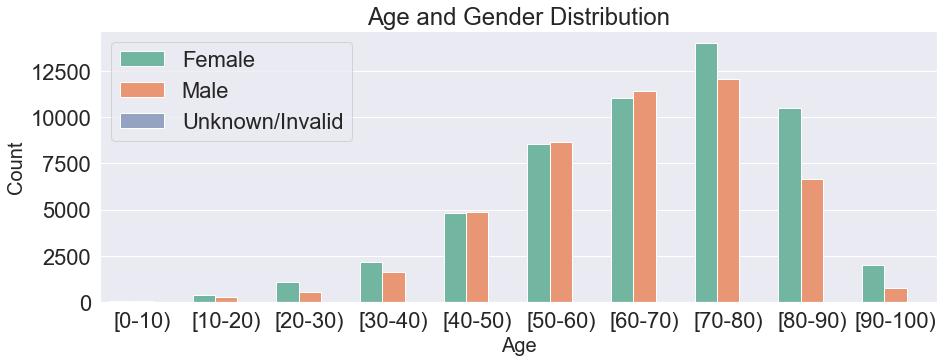
\includegraphics[width=1\linewidth]{../imgs/age_new}
	\caption{Age and Gender Disparity within the dataset}
	\label{fig:age}
\end{figure}

\begin{figure}
	\centering
		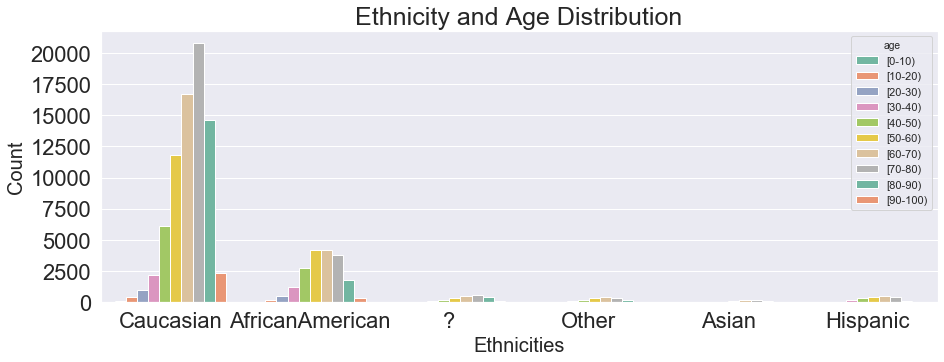
\includegraphics[width=1\linewidth]{../imgs/ethnicities_new}
	\caption{Ethnicity Disparity within the dataset}
	\label{fig:eth}
\end{figure}

Figure \ref{fig:age} and \ref{fig:eth} show that the median age is around 70 to 80 years for diabetes patients, whereas gender can be mostly ignored, because it is almost equally distributed. The ethnicity disparity reveals a bigger concern, because among different ethnicities there is a huge distribution gap. Asians and Hispanics are very underrepresented and African American people in comparison to Caucasian people as well. This plays an important role in the later predictive analysis and explanatory approach. Keeping these distributions in mind, lets with explaining the methods used for this project in respective order:  \\

\begin{itemize}
	\item Model a Neural Network 
	\item Explain the model (\textbf{why}) with Uncertainty Estimation and Metrics
	\item Explain the predictions (\textbf{how}) with SHAP and LIME \\
\end{itemize}


Preprocessing is the first step for modeling a Neural Network. Various unnecessary features needed to be eliminated and categorical features needed to be transformed into a one-hot encoded representation in order to funnel them into the Network properly. The model needs a proper response variable, also called a label, in order to make a proper prediction for the patient selection. I decided on the \textit{time in hospitalization} feature, because it reveals the severity of each patient's diabetes decease. Usually, the longer people need to be hospitalized after receiving treatments, the worse the condition of the person is. So predicting a low hospitalization time with a novel treatment can indicate compatibility with the patient and so he or she is a good match to be selected. 

Neural Networks able to achieve far better results than standard Machine Learning approaches, due to the universal approximation theorem, yet they are less explainable. The Neural Network is modeled with a Keras sequential Neural Network, consisting of Dense, Dropout, Dense Variational and a Distribution Lambda layers to estimate the hospitalization time with a certain probability. The Distribution Lambda layer from Tensorflow incorporates an ensemble of models which report the variability of the prediction. It can be viewed as taking the mean of various regressions and measure the qualitative difference between all outputs. Those layers are implemented to eliminate the risk of: \\

\begin{itemize}
	\item Aleatoric Uncertainty: statisical uncertainty (\textit{known unknowns})
	\item Epistemic Uncertainty systematic uncertainty (\textit{unknown unknowns})\\
\end{itemize}

which usually occurs in clinical data. The aleatoric uncertainty will be evaluated with respect to the ethnicity distribution of the data. The epistemic uncertainty would break the limits of this project.

The neural network's prediction will be measured based on different metrics: \\

\begin{itemize}
	\item Precision, Recall, F1 Score
	\item Brier Score
	\item AUC Score \\
\end{itemize}

The loss function I used was the negativ log likelihood function: 

\begin{center}
	Loss = \(-log(y)\) for each prediction \(y\) \\
\end{center}

The loss generally increases when the regression is unclear and shrinks with more certainty. At this point, the model is now able to predict how long a person is going to stay in the hospital for a specific condition and concerning that person's demographics. The loss has a direct influence on the performance of the metrics. Generally speaking, if the loss is 0, all the metrics are supposed to have a perfect score.

Conclusively to guarantee full transparency of the patient selection process, SHAPely values and LIME try to explain which features led to which output. In other words, which features have a positive and a negative impact on the hospitalization time. The key difference between those two XAI methods is that SHAPely wants to explain \textit{how} the prediction was computed, whereas LIME wants to explain what the most important features were for the prediction.


%
%==================================================
%
\section{Results} 
\begin{figure}
	\centering
	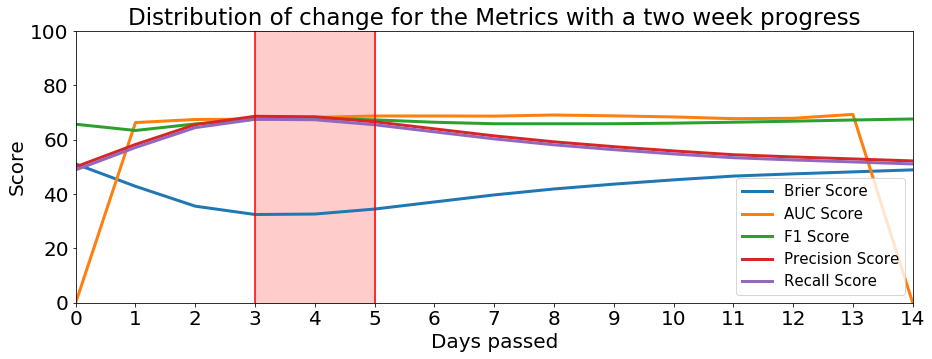
\includegraphics[width=1\linewidth]{../imgs/metrics_time}
	\caption{The graphic shows the temporal change of the metrics with respect to a different time constraint on the boundary. The best values for the metrics can be found within the third and fifth day. Setting the boundary somewhere in the red highlighted area produces the best and most certain estimation.}
	\label{fig:change}
\end{figure}
\noindent After having the workflow in mind, the first step is to train the neural network and evaluate its results. The model trained for 50 epochs and reached a loss of 2.97.  Nevertheless, this alone can not qualify for selecting a patient. There needs to be a specific boundary indicating after which time of hospitalization the diabetes is so serious, that this person can be taken into consideration for the trial, otherwise the selection process can not be accomplished.
Figure \ref{fig:change} shows the course of events for different evaluation metrics. For example the \textit{Brier Score} is best when it is as low as possible, whereas the other scores are best when they are as close to 100 as possible. Taking this into consideration,  if the boundary is set to four on the x-axis, which means four days of hospitalization, all metrics have the globally optimal score. The predictions of the model are closest to the true labels when the boundary is set to four. 
After carefully selecting the most promising discrimination boundary at four days for generating a label, the uncertainty estimation with respect to ethnicity can be computed. \\ \\ \\

\begin{figure}
	\centering
	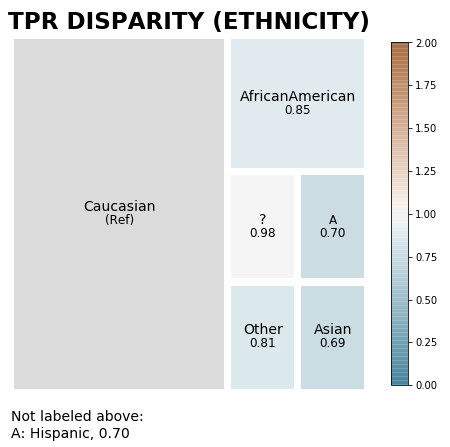
\includegraphics[width=0.8\linewidth]{../imgs/tpr_paper}
	\caption{True positive rate among ethnicities with Caucasiens as reference group with the discrimination boundary at day four}
	\label{fig:tpr}
\end{figure}

\begin{figure}
	\centering
	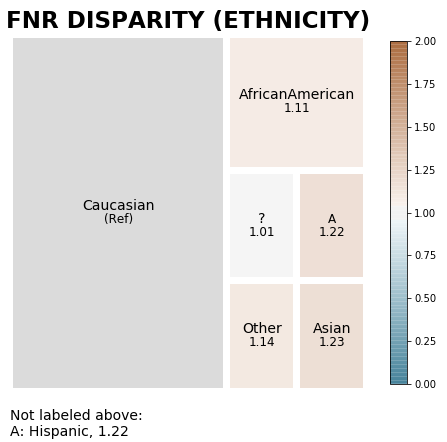
\includegraphics[width=0.8\linewidth]{../imgs/fnr_paper}
	\caption{False negative rate among ethnicities with Caucasiens as reference group with the discrimination boundary at day four}
	\label{fig:fpr}
\end{figure}


Taking a close look at Figures \ref{fig:tpr} and \ref{fig:fpr}, it can be seen that the true positive rate for Caucasian people is higher compared to the other ethnicities. Also, the false-negative rate of other ethnicities is higher compared to the reference Caucasian people. Both indicate, that if a patient is being selected and he or she is Caucasian, the probability of a positive or negative choice is more accurate compared to other ethnicities. Looking back at Figure \ref{fig:eth}, this important prediction disparity can be explained due to the huge difference in training data for all ethnicities. 

The next step is the investigation of how each prediction was computed. As mentioned in the section methods, SHAPely and LIME are used for this purpose. 

\begin{figure}
	\centering
	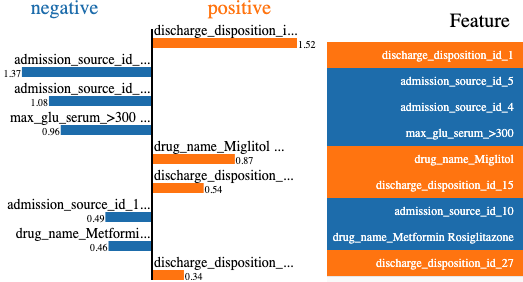
\includegraphics[width=1\linewidth]{../imgs/lime_paper}
	\caption{Important features computed by LIME. The true label for this was 7 days and model predicted a value of 6.42 days.}
	\label{fig:lime}
\end{figure}

Figure \ref{fig:lime} illustrates the single components which led to this prediction of 6.42 days. The categorical features of this prediction can be seen in the following bullet points:  

\begin{itemize}
	\item discharge\_disposition\_id\_1: Discharged to home
	\item admission\_source\_id\_5: Transfer from a Skilled Nursing Facility (SNF)
	\item admission\_source\_id\_4: Transfer from a hospital
	\item admission\_source\_id\_10: Transfer from critial access hospital
\end{itemize}

This specific patient is marked with the features \textit{admission\_type\_id\_1} and \text{discharge\_disposition\_id\_6}. This means that \textbf{not} having the features \text{admission\_source\_id\_5} and \text{6} has an actually \textbf{positive} (fewer days in hospital) impact on the hospitalization time, whereas when a patient has the \textit{discharge\_disposition\_id\_1}, this indicates a longer stay in the hospital. Also e.g. if the patient is taking the medication \textit{Migitol}, he or she generally will stay up to one day (0.87) longer in hospital than people who don't take this drug. Explanations like this can be conducted for all 36 trained on features for further investigation.

\begin{figure}
	\centering
	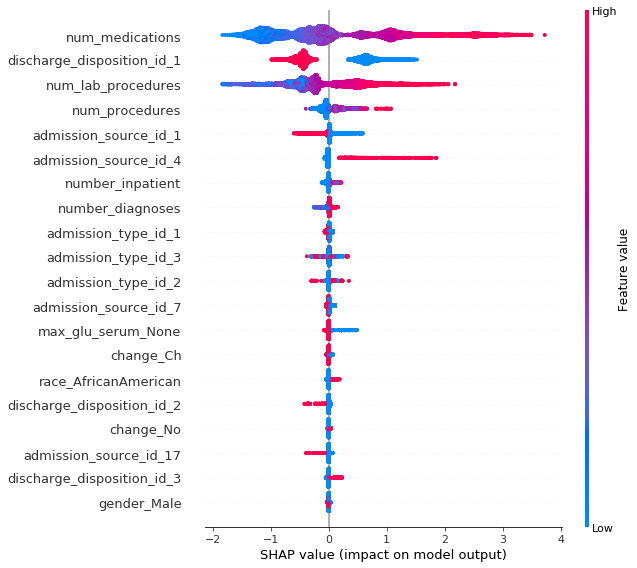
\includegraphics[width=1\linewidth]{../imgs/shap_paper}
	\caption{False negative rate among ethnicities with Caucasiens as reference group with the discrimination boundary at day four}
	\label{fig:shap}
\end{figure}

\begin{figure}
	\centering
	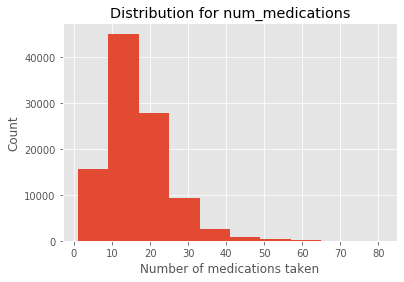
\includegraphics[width=0.9\linewidth]{../imgs/meds_dist}
	\caption{Distribution of the feature \textit{num\_medications}}
	\label{fig:num_meds}
\end{figure}

The second interpretational approach are the SHAPely values, which can be seen in Figure \ref{fig:shap}. This figure lists all features with their distribution on impact for the prediction. For example, the distribution of \textit{num\_medications} can be seen in Figure \ref{fig:num_meds}. This distribution reveals a right-skewed normal distribution. Based on that distribution, it becomes obvious that a normally distributed numerical feature can have both a negative and positive impact on the prediction. The more medications a person takes, the worse the condition and the longer the hospital stay for this person, and vice versa. Whereas the feature \textit{admission\_source\_id\_4}, if marked positive for a person, has always a high positive impact (higher hospitalization time) for the patient.  

%
% === II. 4	Data description with visualization==========================
%
\section{Discussion}
After taking all evaluations and explanatory steps into consideration, can neural networks be applied in the Industry 4.0? There exist many pros and cons. \\

\textbf{Pros}: 

\begin{itemize}
	\item Support for doctor's decision
	\item Patient selection saves a lot of time
	\item Possible new insights \\
\end{itemize}

\textbf{Cons}: 

\begin{itemize}
	\item Unstructured data
	\item Can it also be applied for other EHR data?
	\item Necessary needed data amount is unclear \\
\end{itemize}

I would argue that these techniques can be a good decision-support technology for doctors. If there are for example 2000 patients stored in the hospital database, this selection process can already shrink the number of people that could possibly be suitable for receiving the novel treatment. Doctors will make the final decision based on their experience, but they can end up saving a lot of time by looking at already 20 pre-selected patients instead of investigating 2000 patient files for suitable patients.

 
\section{Conclusion}
\noindent The conclusion of this entire workflow leads to two final questions to be answered. \\

\textit{Apply it without additional doctor’s approval?} \\

For sure not. What if only one person dies because of a false
decision of the neural network's prediction? This is a hot topic and the law and regulatory clinical instances like the FDA in the United States or the Arzneimittelbehörde of Germany comes into force when implementing such technologies in the clinical environment. \\

\textit{Apply it as a support technology?} \\

Sure if a doctor validates the results, it can be used to support the clinical trials and save up a lot of time and identify new interesting insights.

\textit{Does a combination of metrics improve the overall explainability and how many metrics are enough?} \\
Yes. Using first the F1-Score for evaluating the model's performance and then computing the uncertainty estimation with respect to critical features has an overall impro


\section{Future Work}
\noindent For future research further improvements can also be made, such as: \\

\begin{itemize}
	\item Try different XAI methods
	\item Try different Neural Networks or classifiers with GPU?
	\item Epistemic Uncertainty with different Neural Network Layers: tfp.layers.DenseVariational
\end{itemize}


\section*{Acknowledgment}
\noindent Thanks a lot to Philipp Schlieper from the Machine Learning and Data Analytics Lab for a really good supervising through out my project. I can totally recommend this seminar.



% if have a single appendix:
%\appendix[Proof of the Zonklar Equations]
% or
%\appendix  % for no appendix heading
% do not use \section anymore after \appendix, only \section*
% is possibly needed

% use appendices with more than one appendix
% then use \section to start each appendix
% you must declare a \section before using any
% \subsection or using \label (\appendices by itself
% starts a section numbered zero.)
%

% ============================================
%\appendices
%\section{Proof of the First Zonklar Equation}
%Appendix one text goes here %\cite{Roberg2010}.

% you can choose not to have a title for an appendix
% if you want by leaving the argument blank
%\section{}
%Appendix two text goes here.


% use section* for acknowledgement
%\section*{Acknowledgment}


%The authors would like to thank D. Root for the loan of the SWAP. The SWAP that can ONLY be usefull in Boulder...


% Can use something like this to put references on a page
% by themselves when using endfloat and the captionsoff option.
\ifCLASSOPTIONcaptionsoff
  \newpage
\fi



% trigger a \newpage just before the given reference
% number - used to balance the columns on the last page
% adjust value as needed - may need to be readjusted if
% the document is modified later
%\IEEEtriggeratref{8}
% The "triggered" command can be changed if desired:
%\IEEEtriggercmd{\enlargethispage{-5in}}

% ====== REFERENCE SECTION

%\begin{thebibliography}{1}

% IEEEabrv,

\bibliographystyle{IEEEtran}
\bibliography{IEEEabrv,Bibliography}
%\end{thebibliography}
% biography section
% 
% If you have an EPS/PDF photo (graphicx package needed) extra braces are
% needed around the contents of the optional argument to biography to prevent
% the LaTeX parser from getting confused when it sees the complicated
% \includegraphics command within an optional argument. (You could create
% your own custom macro containing the \includegraphics command to make things
% simpler here.)
%\begin{biography}[{\includegraphics[width=1in,height=1.25in,clip,keepaspectratio]{mshell}}]{Michael Shell}
% or if you just want to reserve a space for a photo:

% ==== SWITCH OFF the BIO for submission
% ==== SWITCH OFF the BIO for submission


%% if you will not have a photo at all:
%\begin{IEEEbiographynophoto}{Ignacio Ramos}
%(S'12) received the B.S. degree in electrical engineering from the University of Illinois at Chicago in 2009, and is currently working toward the Ph.D. degree at the University of Colorado at Boulder. From 2009 to 2011, he was with the Power and Electronic Systems Department at Raytheon IDS, Sudbury, MA. His research interests include high-efficiency microwave power amplifiers, microwave DC/DC converters, radar systems, and wireless power transmission.
%\end{IEEEbiographynophoto}

%% insert where needed to balance the two columns on the last page with
%% biographies
%%\newpage

%\begin{IEEEbiographynophoto}{Jane Doe}
%Biography text here.
%\end{IEEEbiographynophoto}
% ==== SWITCH OFF the BIO for submission
% ==== SWITCH OFF the BIO for submission



% You can push biographies down or up by placing
% a \vfill before or after them. The appropriate
% use of \vfill depends on what kind of text is
% on the last page and whether or not the columns
% are being equalized.

\vfill

% Can be used to pull up biographies so that the bottom of the last one
% is flush with the other column.
%\enlargethispage{-5in}



% that's all folks
\end{document}